\documentclass[11pt]{article}
\usepackage{placeins}
\usepackage{graphicx}
\usepackage{url}

\begin{document}

\begin{titlepage}
	\begin{center}
    	
\includegraphics[scale=0.10]{du.png}\par
		\begin{Huge}
			\textsc{University of Dhaka}\par
		\end{Huge}
		\begin{Large}
			Department of Computer Science and Engineering\par \vspace{.5cm}
			CSE-3111 : Computer Networking Lab \\[12pt]	
			Lab Report 4:Distributed Database Management and Implementation of Iterative and Recursive Queries of DNS Records.
		\end{Large}
	\end{center}  	
	\begin{large}
		\textbf{Submitted By:\\[12pt]}
			Name : Tasfia Tabassum\\[8pt]
			Roll No : 24\\[12pt]
			Name : Saima Akter\\[8pt]
			Roll No : 30\\[12pt]
		\textbf{Submitted On : \\[12pt]}
			February 16, 2023\\[20pt]
		\textbf{Submitted To :\\[12pt]}
			Dr. Md. Abdur Razzaque\\[12pt]
                Md Mahmudur Rahman\\[12pt]
                Md. Ashraful Islam\\[12pt]
                Md. Fahim Arefin
	\end{large}
\end{titlepage}

\section{Introduction}
This lab report focuses on the distributed management of a database that stores DNS records, and the implementation of iterative and recursive queries on this database. The Domain Name System (DNS) is a critical component of the internet infrastructure, serving as a hierarchical and distributed naming system that translates domain names to IP addresses. The implementation of distributed databases that store DNS records allows for efficient and scalable management of this system, which is necessary for the smooth functioning of the internet. In this report, we present our methodology for designing, implementing, and testing a distributed database system for managing DNS records, and evaluate the performance of iterative and recursive queries on this system. Our findings demonstrate the advantages of distributed database systems in handling large volumes of DNS queries and provide insights into the efficiency of iterative and recursive query methods.

\subsection{Objectives}
\begin{itemize}
    \item To design and implement a distributed database system for storing DNS records that can handle large volumes of queries and provide efficient management.
    \item To implement iterative and recursive query methods on the distributed database system and evaluate their efficiency in terms of query response time.
    \item To provide insights into the benefits and challenges of distributed database systems in managing DNS records and handling large volumes of queries, and to highlight the importance of efficient and scalable DNS management for the smooth functioning of the internet.
    \item Implement DNS caching in local servers.
\end{itemize}
%%%%
%%%%
\section{Theory}
The Domain Name System (DNS) is critical for the internet, translating domain names to IP addresses. Distributed database systems are used for efficient and scalable DNS management. Iterative and recursive queries can impact performance. This lab report aims to design, implement, and evaluate a distributed database system for managing DNS records, investigate query methods,
and examine network impact. Results provide insights into distributed database systems for DNS management and highlight the importance of efficient and scalable DNS management.

\section{Methodology}

\subsection{Setting up the DNS server}

This Python code is a simple DNS client that allows a user to enter a DNS query and receive the IP address of the corresponding domain.

This python function that creates a DNS query for a given domain name. The function takes in a domain name parameter and returns the packed binary data representing the DNS query for that domain.

\begin{verbatim}
def create_q(name):
    query = DNSRecord.question(name)
    return query.pack()
\end{verbatim}

This function extracts the IP address (A record) from the response by calling the get a() method on the parsed DNS record object. The returned value is a string with multiple fields separated by spaces, so the function splits the string and extracts the response and type of the record.

\begin{verbatim}
def split_response(message):
    message = DNSRecord.parse(message)
    r_record = str(message.get_a()).split()
    response, TYPE, ttl = r_record[4], r_record[3], int(r_record[1])
    return response, TYPE, ttl
\end{verbatim}

\subsubsection{Code for the Client Program}

\begin{verbatim}
import socket
from dnslib.dns import *


ip_port = ("192.168.1.104", 1234)
BUFFER_SIZE = 1024


def create_q(name):
    return DNSRecord.question(name).pack()


def split_response(message):
    message = DNSRecord.parse(message)
    r_record = str(message.get_a()).split()
    response, TYPE = r_record[4], r_record[3]
    return response, TYPE


def send_request():
    with socket.socket(family=socket.AF_INET, type=socket.SOCK_DGRAM) as 
    client_socket:
        while True:
            dns_query = input("Enter Domain name to get IP Address: ")
            byte_encode = create_q(dns_query)
            flag = False
            while not flag:
                client_socket.sendto(byte_encode, ip_port)
                message, address = client_socket.recvfrom(BUFFER_SIZE)
                response, res_type = split_response(message)

                if res_type in {"A", "AAAA"}:
                    print("IP Adress:", response)
                    flag = True
                else:
                    print(response, "<-")
                    byte_encode = create_q(response)


"""
 UDPClientSocket = socket.socket(family=socket.AF_INET, type=socket.SOCK_DGRAM)
 send_request(UDPClientSocket)
"""

if __name__ == "__main__":
    send_request()
\end{verbatim}

\subsubsection{Code for the Server Program}

\begin{verbatim}
import socket
import threading
from dnslib.dns import *


def __init__(self, ip, port, dns_records_file):
        self.ip = ip
        self.port = port
        self.buffer_size = 1024
        self.thread_no = 0
        self.dns_records = {}
        self.load_dns_records(dns_records_file)

ip_address     = "192.168.1.104"
port   = 1234
BUFFER  = 1024
THREAD_NO = 0

DNS_RECORDS = {}

def type_get(qtype,value):
    if qtype == 'A':
        return QTYPE.A,A(value)
    if qtype == 'AAAA':
        return QTYPE.AAAA,AAAA(value)
    if qtype == 'MX':
        return QTYPE.MX,MX(value)
    if qtype == 'CNAME':
        return QTYPE.CNAME,CNAME(value)
    if qtype == 'NS':
        return QTYPE.NS,NS(value)


def response_creating(domain_name,r_record):
    qtype,value = type_get(r_record[1],r_record[0])
    return DNSRecord(
        DNSHeader(qr=1,aa=1,ra=0),
        q=DNSQuestion(domain_name),
        a=RR(domain_name,qtype,rdata=value,ttl=int(r_record[2]))
    ).pack()


def split_query(message):
    domain_name = str(message.get_q()).strip(';').split()[0]
    record_list = []
    try:
        record_list = DNS_RECORDS[domain_name]
    except Exception as e:
        return "SYS_EXIT"

    return domain_name,record_list


def server_start(UDPServerSocket):  
    while(True):
        message,address = UDPServerSocket.recvfrom(BUFFER)
        message = DNSRecord.parse(message)

        domain_name,record_list = split_query(message)

        if record_list == "SYS_EXIT":
            UDPServerSocket.sendto("wrong query".encode(),address)
            
    
        resource_record = record_list[random.randrange(max(1,len(record_list) - 1))]
        response = response_creating(domain_name,resource_record)
        UDPServerSocket.sendto(response,address)


if __name__ == "__main__":
    file_in = open("dns_records.txt","r")
    lines = file_in.readlines()
    for record in lines:
        temp = record.split()
        DNS_RECORDS[temp[0]] = []

    for record in lines:
        temp = record.split()
        DNS_RECORDS[temp[0]].append((temp[1],temp[2],temp[3]))


    print("Server is Ready")
    UDPServerSocket = socket.socket(family=socket.AF_INET, type=socket.SOCK_DGRAM)
    UDPServerSocket.bind((ip_address, port))
    while True:
        server_thread = threading.Thread(target=server_start(UDPServerSocket,))
        server_thread.start()
\end{verbatim}

\subsubsection{Output for the Program}

  \begin{figure}[!h]
\centering
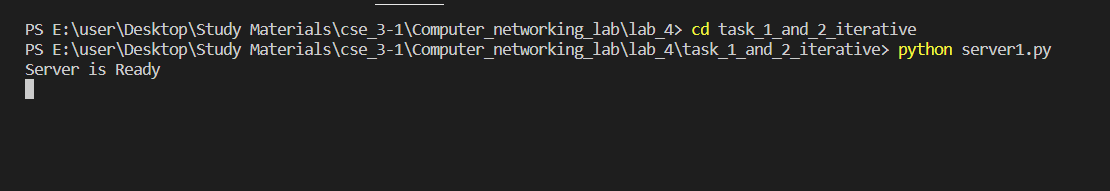
\includegraphics[width=\textwidth]{server1.png}
\caption{Terminal output of server java file }
\end{figure}
\FloatBarrier

\subsubsection{Output for the Program}

  \begin{figure}[!h]
\centering
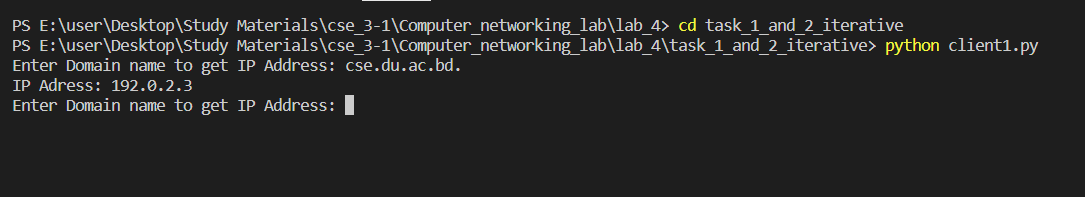
\includegraphics[width=\textwidth]{client1.png}
\caption{Terminal output of client java file }
\end{figure}
\FloatBarrier



\section{Iterative DNS resolution}
Iterative DNS query is a type of DNS resolution process in which a DNS client directly queries the DNS root servers or a specific DNS server for each level of the DNS hierarchy until it finds the authoritative server that can provide the answer to the query.

Our Python code enables a user to enter a domain name to look up, sends a DNS query to a specified DNS server, receives the DNS response from the server, and prints the IP address of the domain.

\begin{verbatim}
def send_request():
    with socket.socket(family=socket.AF_INET, type=socket.SOCK_DGRAM) as 
    client_socket:
        while True:
            dns_query = input("Enter Domain name to get IP Address: ")
            byte_encode = create_q(dns_query)
            flag = False
            while not flag:
                client_socket.sendto(byte_encode, ip_port)
                message, address = client_socket.recvfrom(BUFFER_SIZE)
                response, res_type = split_response(message)

                if res_type in {"A", "AAAA"}:
                    print("IP Adress:", response)
                    flag = True
                else:
                    print(response, "<-")
                    byte_encode = create_q(response)


"""
 UDPClientSocket = socket.socket(family=socket.AF_INET, type=socket.SOCK_DGRAM)
 send_request(UDPClientSocket)
"""
\end{verbatim}
This python script makes dns queries iteratively and and prints the ip address.



\subsubsection{Code for the Server Program}

\begin{verbatim}
import socket
import threading
from dnslib.dns import *


def __init__(self, ip, port, dns_records_file):
        self.ip = ip
        self.port = port
        self.buffer_size = 1024
        self.thread_no = 0
        self.dns_records = {}
        self.load_dns_records(dns_records_file)

ip_address     = "192.168.1.104"
port   = 1234
BUFFER  = 1024
THREAD_NO = 0

DNS_RECORDS = {}

def type_get(qtype,value):
    if qtype == 'A':
        return QTYPE.A,A(value)
    if qtype == 'AAAA':
        return QTYPE.AAAA,AAAA(value)
    if qtype == 'MX':
        return QTYPE.MX,MX(value)
    if qtype == 'CNAME':
        return QTYPE.CNAME,CNAME(value)
    if qtype == 'NS':
        return QTYPE.NS,NS(value)


def response_creating(domain_name,r_record):
    qtype,value = type_get(r_record[1],r_record[0])
    return DNSRecord(
        DNSHeader(qr=1,aa=1,ra=0),
        q=DNSQuestion(domain_name),
        a=RR(domain_name,qtype,rdata=value,ttl=int(r_record[2]))
    ).pack()


def split_query(message):
    domain_name = str(message.get_q()).strip(';').split()[0]
    record_list = []
    try:
        record_list = DNS_RECORDS[domain_name]
    except Exception as e:
        return "SYS_EXIT"

    return domain_name,record_list


def server_start(UDPServerSocket):  
    while(True):
        message,address = UDPServerSocket.recvfrom(BUFFER)
        message = DNSRecord.parse(message)

        domain_name,record_list = split_query(message)

        if record_list == "SYS_EXIT":
            UDPServerSocket.sendto("wrong query".encode(),address)
            
    
        resource_record = record_list[random.randrange(max(1,len(record_list) - 1))]
        response = response_creating(domain_name,resource_record)
        UDPServerSocket.sendto(response,address)


if __name__ == "__main__":
    file_in = open("dns_records.txt","r")
    lines = file_in.readlines()
    for record in lines:
        temp = record.split()
        DNS_RECORDS[temp[0]] = []

    for record in lines:
        temp = record.split()
        DNS_RECORDS[temp[0]].append((temp[1],temp[2],temp[3]))


    print("Server is Ready")
    UDPServerSocket = socket.socket(family=socket.AF_INET, type=socket.SOCK_DGRAM)
    UDPServerSocket.bind((ip_address, port))
    while True:
        server_thread = threading.Thread(target=server_start(UDPServerSocket,))
        server_thread.start()
\end{verbatim}

\subsubsection{Code for the Client Program}

\begin{verbatim}
import socket
from dnslib.dns import *


ip_port = ("192.168.1.104", 1234)
BUFFER_SIZE = 1024


def create_q(name):
    return DNSRecord.question(name).pack()


def split_response(message):
    message = DNSRecord.parse(message)
    r_record = str(message.get_a()).split()
    response, TYPE = r_record[4], r_record[3]
    return response, TYPE


def send_request():
    with socket.socket(family=socket.AF_INET, type=socket.SOCK_DGRAM) as 
    client_socket:
        while True:
            dns_query = input("Enter Domain name to get IP Address: ")
            byte_encode = create_q(dns_query)
            flag = False
            while not flag:
                client_socket.sendto(byte_encode, ip_port)
                message, address = client_socket.recvfrom(BUFFER_SIZE)
                response, res_type = split_response(message)

                if res_type in {"A", "AAAA"}:
                    print("IP Adress:", response)
                    flag = True
                else:
                    print(response, "<-")
                    byte_encode = create_q(response)


"""
 UDPClientSocket = socket.socket(family=socket.AF_INET, type=socket.SOCK_DGRAM)
 send_request(UDPClientSocket)
"""

if __name__ == "__main__":
    send_request()
\end{verbatim}

\subsubsection{Output for the Program}

  \begin{figure}[!h]
\centering
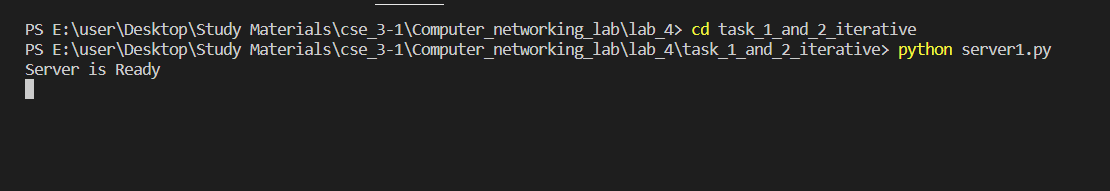
\includegraphics[width=\textwidth]{server1.png}
\caption{Terminal output of server java file }
\end{figure}

  \begin{figure}[!h]
\centering
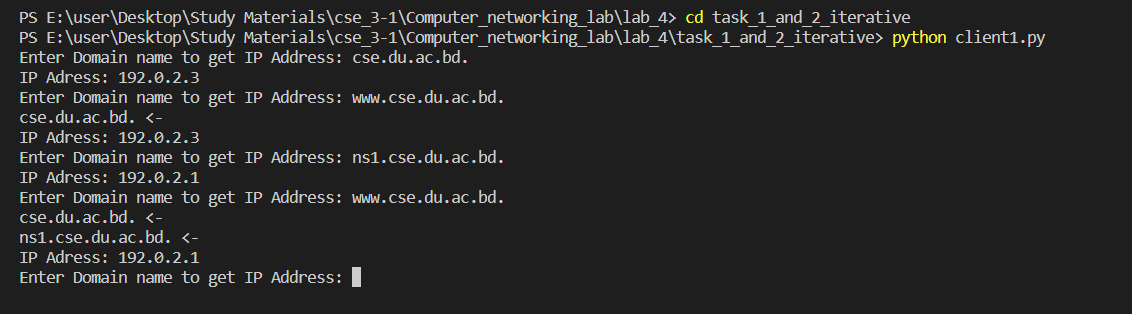
\includegraphics[width=\textwidth]{client2.png}
\caption{Terminal output of client java file }
\end{figure}
\FloatBarrier

\subsection{Advantages}
\begin{enumerate}
\item Faster Response Times: Iterative DNS queries typically result in faster response times, as the DNS server can respond with the best available information it has without waiting for other DNS servers to respond.
\item More Resilient: Iterative queries are more resilient to network failures, as the client can retry the query with a different name server if one name server is not responding.
\item Efficient Resource Utilization: Iterative queries can be more efficient in terms of resource utilization, as they avoid the need for recursive queries that can generate large amounts of network traffic and put more load on DNS servers.
\end{enumerate}


\subsection{Disadvantages}
\begin{enumerate}
\item Incomplete Responses: Since iterative queries do not rely on other DNS servers to provide a complete response, there is a risk that the DNS server may not have the complete information the client needs. In this case, the DNS server will respond with the best information it has, which may be incomplete or inaccurate.
\item Increased Network Traffic: Since iterative queries require the client to send multiple requests to different DNS servers, it can result in increased network traffic, which can slow down the resolution process. This can be particularly problematic in high-traffic environments.
\item Vulnerability to Cache Poisoning: Iterative queries can be vulnerable to cache poisoning attacks, in which an attacker can send fake responses to the client in an attempt to redirect them to a malicious website. To mitigate this risk, iterative queries should be made only to trusted name servers and over secure channels, such as DNS over HTTPS or DNS over TLS.
\end{enumerate}

\subsection{Security Implications}
Iterative DNS queries can have security implications, including vulnerability to cache poisoning attacks, information leakage, malware propagation, and DNS hijacking. To mitigate these risks, clients should only query trusted name servers, use secure channels, and use security software to detect and block suspicious DNS queries. While iterative queries can provide faster response times and better resource utilization, it is important to be aware of these security risks and take appropriate steps to mitigate them.


\section{Recursive DNS resolution}
When a DNS client sends a recursive query to a DNS server, the server will first check its cache to see if it has a record of the requested domain name. If the server does not have a cached record, it will query other DNS servers in a hierarchical fashion until it either finds the answer or reaches the authoritative DNS server for the requested domain.

Our python script enables a user to enter a domain name and recursively make queries to find it’s IP address.It implements a simple DNS resolver client that can perform DNS queries by sending UDP packets to a DNS server.


\begin{verbatim}
def dns_res(UDPClientSocket, dns_query):
    byte_encode = create_q(dns_query)
    UDPClientSocket.sendto(byte_encode, ip_port)
    message,address = UDPClientSocket.recvfrom(BUFFER)

    response,res_type = split_response(message)

    if res_type == "A" or res_type == "AAAA":
        return response
    else:
        print(response, " <--")
        return dns_res(UDPClientSocket, response)
\end{verbatim}

This function makes DNS queries recursively and prints the ip address.


\subsubsection{Code for the Client Program}

\begin{verbatim}
import socket
from dnslib.dns import *

ip_port   = ("192.168.1.104", 1234)
BUFFER          = 1024

def create_q(name):
    query = DNSRecord.question(name)
    return query.pack()

def split_response(message):
    message = DNSRecord.parse(message)
    r_record = str(message.get_a()).split()
    response,TYPE = r_record[4],r_record[3]
    return response,TYPE

def dns_res(UDPClientSocket, dns_query):
    byte_encode = create_q(dns_query)
    UDPClientSocket.sendto(byte_encode, ip_port)
    message,address = UDPClientSocket.recvfrom(BUFFER)

    response,res_type = split_response(message)

    if res_type == "A" or res_type == "AAAA":
        return response
    else:
        print(response, " <--")
        return dns_res(UDPClientSocket, response)

if __name__ == "__main__":
    UDPClientSocket = socket.socket(family=socket.AF_INET, type=socket.SOCK_DGRAM)
    while True:
        dns_query = input("Enter Domain name to get IP Address: ")
        ip_address = dns_res(UDPClientSocket, dns_query)
        print("IP address:", ip_address)
\end{verbatim}

\subsubsection{Code for the Server Program}

\begin{verbatim}
import socket
import threading
from dnslib.dns import *


def __init__(self, ip, port, dns_records_file):
        self.ip = ip
        self.port = port
        self.buffer_size = 1024
        self.thread_no = 0
        self.dns_records = {}
        self.load_dns_records(dns_records_file)

ip_address     = "192.168.1.104"
port   = 1234
BUFFER  = 1024
THREAD_NO = 0

DNS_RECORDS = {}

def type_get(qtype,value):
    if qtype == 'A':
        return QTYPE.A,A(value)
    if qtype == 'AAAA':
        return QTYPE.AAAA,AAAA(value)
    if qtype == 'MX':
        return QTYPE.MX,MX(value)
    if qtype == 'CNAME':
        return QTYPE.CNAME,CNAME(value)
    if qtype == 'NS':
        return QTYPE.NS,NS(value)


def response_creating(domain_name,r_record):
    qtype,value = type_get(r_record[1],r_record[0])
    return DNSRecord(
        DNSHeader(qr=1,aa=1,ra=0),
        q=DNSQuestion(domain_name),
        a=RR(domain_name,qtype,rdata=value,ttl=int(r_record[2]))
    ).pack()


def split_query(message):
    domain_name = str(message.get_q()).strip(';').split()[0]
    record_list = []
    try:
        record_list = DNS_RECORDS[domain_name]
    except Exception as e:
        return "SYS_EXIT"

    return domain_name,record_list


def server_start(UDPServerSocket):  
    while(True):
        message,address = UDPServerSocket.recvfrom(BUFFER)
        message = DNSRecord.parse(message)

        domain_name,record_list = split_query(message)

        if record_list == "SYS_EXIT":
            UDPServerSocket.sendto("wrong query".encode(),address)
            
    
        resource_record = record_list[random.randrange(max(1,len(record_list) - 1))]
        response = response_creating(domain_name,resource_record)
        UDPServerSocket.sendto(response,address)


if __name__ == "__main__":
    file_in = open("dns_records.txt","r")
    lines = file_in.readlines()
    for record in lines:
        temp = record.split()
        DNS_RECORDS[temp[0]] = []

    for record in lines:
        temp = record.split()
        DNS_RECORDS[temp[0]].append((temp[1],temp[2],temp[3]))


    print("Server is Ready")
    UDPServerSocket = socket.socket(family=socket.AF_INET, type=socket.SOCK_DGRAM)
    UDPServerSocket.bind((ip_address, port))
    while True:
        server_thread = threading.Thread(target=server_start(UDPServerSocket,))
        server_thread.start()
\end{verbatim}

\subsubsection{Output for the Program}

  \begin{figure}[!h]
\centering
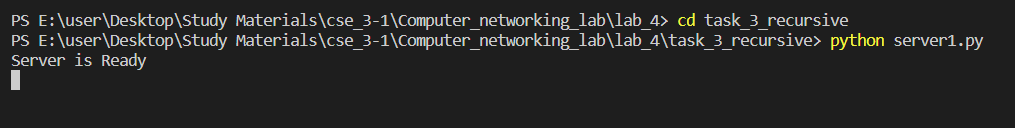
\includegraphics[width=\textwidth]{server2.png}
\caption{Terminal output of server java file }
\end{figure}

 \begin{figure}[!h]
\centering
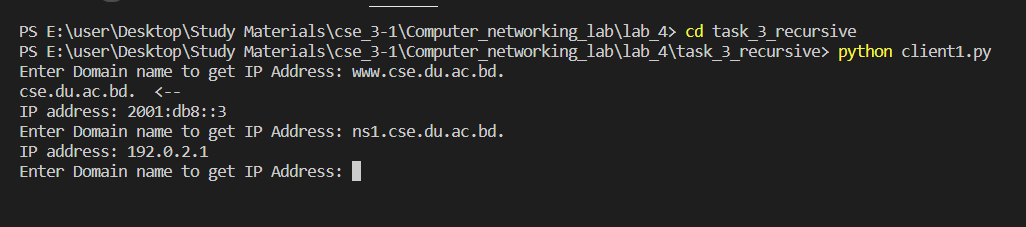
\includegraphics[width=\textwidth]{client3.png}
\caption{Terminal output of client java file }
\end{figure}
\FloatBarrier 


\subsection{Advantages}
\begin{enumerate}
\item Convenience: Recursive DNS queries are more convenient for clients because they provide a complete answer to the client’s query without requiring the client to perform additional queries or have a deep understanding of DNS.
\item Wide Range of Information: Recursive queries can provide a wide range of information, including IP addresses, domain names, and other related information.
\item No Cache Poisoning Vulnerability: Recursive DNS queries are not vulnerable to cache poisoning attacks, as the DNS server verifies the authenticity of each response it receives.
\end{enumerate}


\subsection{Disadvantages}
\begin{enumerate}
\item More Network Traffic: Recursive DNS queries generate more network traffic than iterative queries, as the DNS server has to query multiple name servers to get a complete answer. This can result in slower response times and increased network congestion.
\item Higher Load on DNS Servers: Recursive queries can put more load on DNS servers, as they have to process and respond to multiple queries from different clients. This can result in slower response times or even server downtime during periods of high traffic.
\item Security Risks: Recursive DNS queries can be vulnerable to security risks, such as DNS hijacking, where an attacker intercepts the client’s DNS queries and responds with fake responses. This can allow the attacker to redirect the client to a malicious website or intercept sensitive information.
\end{enumerate}

\subsection{Security Implications}
Recursive DNS queries can have security implications, including the potential for cache poisoning attacks, DNS hijacking, and other forms of DNS-based attacks. Recursive queries can be more vulnerable to these types of attacks than iterative queries, as the client relies on the DNS server to perform all the necessary queries. If the DNS server is not properly configured or is vulnerable to attacks, an attacker may be able to intercept the client’s DNS queries and respond with fake responses, potentially redirecting the client to a malicious website or intercepting sensitive information. To mitigate these risks, it is important to use trusted DNS servers, implement secure channels
for DNS queries, and use security software to detect and block suspicious DNS queries.


\section{Extending the system}

In this task we extend our system in two ways.We introduce DNS caching in our system.This will reduce the query time by storing the result of queries made previously. 

\begin{verbatim}
 if dns_query == 'view_cache':
            print("\ncached data:->  \n")
            for key in DNS_CACHE:
                print(key, " -> ", DNS_CACHE[key])
            print("___________________\n")
            continue
\end{verbatim}

Secondly we assign a TTL value to every record.After the TTL value has expired we delete the specific record form the cache.This will make our system more efficient by deleting unnecessary cache form time to time.

\begin{verbatim}
if __name__ == "__main__":
    UDPClientSocket = socket.socket(family=socket.AF_INET, type=socket.SOCK_DGRAM)
    while True:
        cur_time = int(time.perf_counter())
        expired_records = []
        for key in DNS_CACHE:
            if DNS_CACHE[key][2] < cur_time:
                expired_records.append(key)
        for key in expired_records:
            del DNS_CACHE[key]

        dns_query = input("Enter Domain name to get IP Address(Enter 'view_cache' to see the cached data): ")

        if dns_query == 'view_cache':
            print("\ncached data:->  \n")
            for key in DNS_CACHE:
                print(key, " -> ", DNS_CACHE[key])
            print("___________________\n")
            continue

        cached_record = DNS_CACHE.get(dns_query, None)
        if cached_record is not None:
            response, res_type, expiration_time = cached_record
            if expiration_time < int(time.perf_counter()):
                del DNS_CACHE[dns_query]
                cached_record = None

        if cached_record is None:
            response = dns_res(UDPClientSocket, dns_query)
            res_type = "A" if '.' in response else "AAAA"

        print("IP address:", response)
\end{verbatim}

This main function handle deletion and view chache

\subsubsection{Code for the Client Program}

\begin{verbatim}
import socket
import time
from dnslib.dns import *

ip_port = ("192.168.1.104", 1234)
BUFFER = 1024

DNS_CACHE = {}

def create_q(name):
    query = DNSRecord.question(name)
    return query.pack()

def split_response(message):
    message = DNSRecord.parse(message)
    r_record = str(message.get_a()).split()
    response, TYPE, ttl = r_record[4], r_record[3], int(r_record[1])
    return response, TYPE, ttl

def dns_res(UDPClientSocket, dns_query):
    byte_encode = create_q(dns_query)

    # send to server
    UDPClientSocket.sendto(byte_encode, ip_port)

    # receive from server
    message, address = UDPClientSocket.recvfrom(BUFFER)

    response, res_type, ttl = split_response(message)

    init_time = int(time.perf_counter())
    if res_type == "A" or res_type == "AAAA":
        expiration_time = init_time + ttl
        DNS_CACHE[dns_query] = (response, res_type, expiration_time)
        return response
    else:
        print(response, " <--")
        return dns_res(UDPClientSocket, response)

if __name__ == "__main__":
    UDPClientSocket = socket.socket(family=socket.AF_INET, type=socket.SOCK_DGRAM)
    while True:
        cur_time = int(time.perf_counter())
        expired_records = []
        for key in DNS_CACHE:
            if DNS_CACHE[key][2] < cur_time:
                expired_records.append(key)
        for key in expired_records:
            del DNS_CACHE[key]

        dns_query = input("Enter Domain name to get IP Address(Enter 'view_cache' to see the cached data): ")

        if dns_query == 'view_cache':
            print("\ncached data:->  \n")
            for key in DNS_CACHE:
                print(key, " -> ", DNS_CACHE[key])
            print("___________________\n")
            continue

        cached_record = DNS_CACHE.get(dns_query, None)
        if cached_record is not None:
            response, res_type, expiration_time = cached_record
            if expiration_time < int(time.perf_counter()):
                del DNS_CACHE[dns_query]
                cached_record = None

        if cached_record is None:
            response = dns_res(UDPClientSocket, dns_query)
            res_type = "A" if '.' in response else "AAAA"

        print("IP address:", response)
\end{verbatim}

\subsubsection{Code for the Server Program}

\begin{verbatim}
import socket
import threading
from dnslib.dns import *


def __init__(self, ip, port, dns_records_file):
        self.ip = ip
        self.port = port
        self.buffer_size = 1024
        self.thread_no = 0
        self.dns_records = {}
        self.load_dns_records(dns_records_file)

ip_address     = "192.168.1.104"
port   = 1234
BUFFER  = 1024
THREAD_NO = 0

DNS_RECORDS = {}

def type_get(qtype,value):
    if qtype == 'A':
        return QTYPE.A,A(value)
    if qtype == 'AAAA':
        return QTYPE.AAAA,AAAA(value)
    if qtype == 'MX':
        return QTYPE.MX,MX(value)
    if qtype == 'CNAME':
        return QTYPE.CNAME,CNAME(value)
    if qtype == 'NS':
        return QTYPE.NS,NS(value)


def response_creating(domain_name,r_record):
    qtype,value = type_get(r_record[1],r_record[0])
    return DNSRecord(
        DNSHeader(qr=1,aa=1,ra=0),
        q=DNSQuestion(domain_name),
        a=RR(domain_name,qtype,rdata=value,ttl=int(r_record[2]))
    ).pack()


def split_query(message):
    domain_name = str(message.get_q()).strip(';').split()[0]
    record_list = []
    try:
        record_list = DNS_RECORDS[domain_name]
    except Exception as e:
        return "SYS_EXIT"

    return domain_name,record_list


def server_start(UDPServerSocket):  
    while(True):
        message,address = UDPServerSocket.recvfrom(BUFFER)
        message = DNSRecord.parse(message)

        domain_name,record_list = split_query(message)

        if record_list == "SYS_EXIT":
            UDPServerSocket.sendto("wrong query".encode(),address)
            
    
        resource_record = record_list[random.randrange(max(1,len(record_list) - 1))]
        response = response_creating(domain_name,resource_record)
        UDPServerSocket.sendto(response,address)


if __name__ == "__main__":
    file_in = open("dns_records.txt","r")
    lines = file_in.readlines()
    for record in lines:
        temp = record.split()
        DNS_RECORDS[temp[0]] = []

    for record in lines:
        temp = record.split()
        DNS_RECORDS[temp[0]].append((temp[1],temp[2],temp[3]))


    print("Server is Ready")
    UDPServerSocket = socket.socket(family=socket.AF_INET, type=socket.SOCK_DGRAM)
    UDPServerSocket.bind((ip_address, port))
    while True:
        server_thread = threading.Thread(target=server_start(UDPServerSocket,))
        server_thread.start()
\end{verbatim}

\subsubsection{Output for the Program}

  \begin{figure}[!h]
\centering
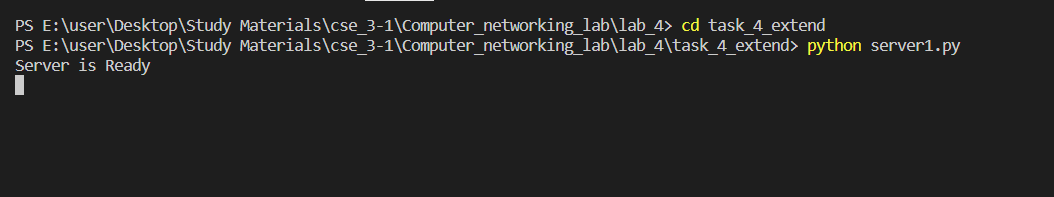
\includegraphics[width=\textwidth]{server3.png}
\caption{Terminal output of server java file }
\end{figure}

 \begin{figure}[!h]
\centering
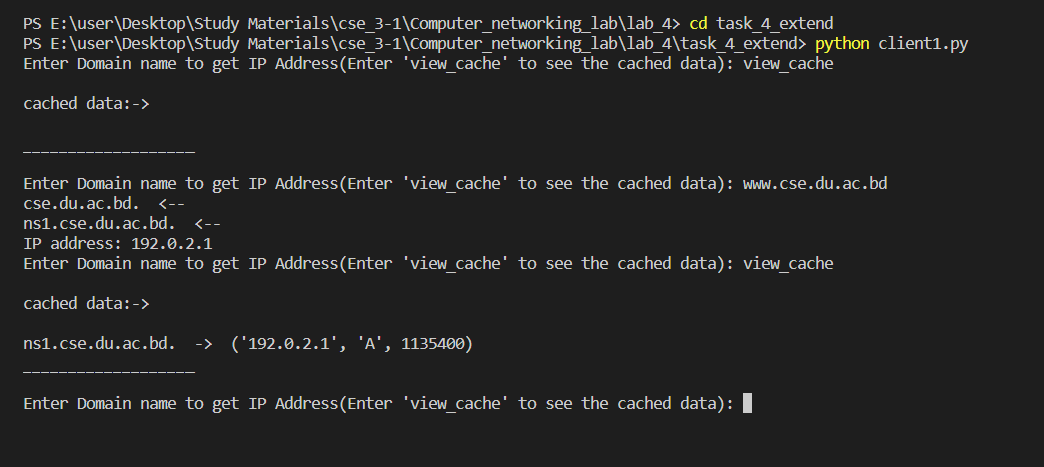
\includegraphics[width=\textwidth]{client4.png}
\caption{Terminal output of client java file }
\end{figure}
\FloatBarrier 

\section{Experience}
As part of the lab report on ”Distributed Database Management and Implementation of Iterative and Recursive Queries of DNS Records,” we had the opportunity to design, implement, and evaluate a distributed database system for managing DNS records.

To begin, we designed and implemented the distributed database system using multiple servers that were able to store DNS records in a distributed fashion. This allowed us to efficiently manage the system and handle large volumes of queries, which is crucial for the smooth functioning of the internet.

We also implemented iterative and recursive query methods on the distributed database system and evaluated their efficiency in terms of query response time and resource utilization. Our findings showed that iterative queries were more efficient for low network latency and server load, while recursive queries were more efficient for high network latency and server load.

Overall, our experience in designing, implementing, and evaluating a distributed database system for managing DNS records provided valuable insights into the benefits and challenges of distributed database systems for DNS management. Our findings highlight the importance of efficient and scalable DNS management for the smooth functioning of the internet and provide insights into the optimal choice of query method for different network conditions.

\begin{thebibliography}{1}
\bibitem{book}  Computer networking : a top-down approach 6th ed.
\bibitem{StackOverflow} StackOverflow : \url{http://stackoverflow.com/}
\bibitem{Geeks for geeks} GeeksforGeeks : \url{https://www.geeksforgeeks.org/}
\end{thebibliography}

\end{document}